\begin{savequote}[45mm]
\ascii{Any fool can write code that a computer can understand. Good programmers write code that humans can understand.}
\qauthor{\ascii{- Martin Flower}}
\end{savequote}

\chapter{解耦合} 
\label{ch:decoupling}

\begin{content}

\end{content}

\section{关键抽象}

\begin{content}

分析\ascii{TestCase::protect}实现,它间接调用\ascii{TestCase}的成员函数\ascii{setUp, runTest, tearDown},而异常处理逻辑主要分布于\ascii{TestResult}的成员函数\ascii{addFailure, addError}。从代码职责分布看,\ascii{TestCase::protect}主要完成异常处理逻辑,与\ascii{TestResult}关系更加紧密。

\begin{nodiff}{src/mars/core/TestCase.cc}
 \begin{c++}
#include <mars/core/TestCase.h>
#include <mars/core/TestResult.h>
#include <mars/except/AssertionError.h>

bool TestCase::protect(TestResult& result, Method method) {
  bool succ = false;
  try {
    (this->*method)();
    succ = true;
  } catch (const AssertionError&) {
    result.addFailure();
  } catch (const std::exception&) {
    result.addError();
  } catch (...) {
    result.addError();
  }
  return succ;
}

void TestCase::run(TestResult& result) {
  if (protect(result, &TestCase::setUp)) {
    protect(result, &TestCase::runTest);
  }
  protect(result, &TestCase::tearDown);
}
 \end{c++}
\end{nodiff}

根据迪米特法则,这段异常处理的逻辑应搬迁至\ascii{TestResult}。当捕获异常后,直接更新到自己的私有数据域,实现\ascii{TestResult::addFailure, TestResult::addError}监听接口的私有化。但是,如果搬迁\ascii{protect}逻辑到\ascii{TestResult},那么\ascii{TestResult}如何调用到\ascii{TestCase}的成员函数\ascii{setUp, runTest, tearDown}呢?

此时似乎陷入窘境,因为\ascii{TestCase}与\ascii{TestResult}之间的耦合太过紧密,拆分显得不是那么容易。因此,解除\ascii{TestCase}与\ascii{TestResult}之间的耦合迫在眉睫。

\subsection{函数式接口}

为了彻底解开\ascii{protect}对\ascii{TestCase}的依赖,引入关键抽象\ascii{TestCaseFunctor},相对\ascii{TestCase::Method}的简单抽象,它不包含\ascii{TestCase}的任何信息,可以与之彻底解耦。因此,\ascii{TestCaseFunctor}更加稳定、更加具有可扩展性\footnote{例如,通过增加\ascii{getTestName}接口,可以携带更多元数据。}。

\ascii{using}或\ascii{typedef}的别名机制,功能单一,抽象能力有限。最重要的是,此处它强度依赖于\ascii{TestCase}的类型信息,两者存在隐式的耦合关系。

\begin{diff}{include/mars/core/internal/TestCaseFunctor.h}
 \begin{minicpp}
using Method = void(TestCase::*)();
 \end{minicpp}
\tcblower
 \begin{minicpp}
struct TestCaseFunctor {
  virtual bool operator()() const = 0;
  virtual ~TestCaseFunctor() {}
};
 \end{minicpp}
\end{diff}

\subsection{实现抽象}

在\ascii{TestCase.h}的文件中,修改\ascii{TestCase::protect}的声明,让其依赖于更稳定的抽象\ascii{TestCaseFunctor},而非简单抽象\ascii{TestCase::Method}。

\begin{diff}{include/mars/core/TestCase.h}
 \begin{minicpp}
#include <mars/core/Test.h>
#include <mars/core/TestFixture.h>

struct TestCase : Test, private TestFixture {
  using Test::Test;

private:
  void run(TestResult&) override;
  int countTestCases() const override;

private:
  virtual void runTest() {}

private:
  using Method = void(TestCase::*)();
  bool protect(TestResult& result, Method method);
};
 \end{minicpp}
\tcblower
 \begin{minicpp}
#include <mars/core/Test.h>
#include <mars/core/TestFixture.h>

struct TestCaseFunctor;

struct TestCase : Test, private TestFixture {
  using Test::Test;

private:
  void run(TestResult&) override;
  int countTestCases() const override;

private:
  virtual void runTest() {}

private:
  bool protect(TestResult&, const TestCaseFunctor&);
}; 
  \end{minicpp}
\end{diff}

在\ascii{TestCase.cc}实现文件中,在匿名命名空间内定义实现\ascii{Functor},它是\ascii{TestCaseFunctor}背后运行的真正实现,它封装实现了原来\ascii{TestCase::Method}的间接调用。

\begin{diff}{src/mars/core/TestCase.cc}
 \begin{minicpp}
#include <mars/core/TestCase.h>
#include <mars/core/TestResult.h>
#include <mars/except/AssertionError.h>

bool TestCase::protect
  (TestResult& result, Method method) {
  bool succ = false;
  try {
    (this->*method)();
    succ = true;
  } catch (const AssertionError&) {
    result.addFailure();
  } catch (const std::exception&) {
    result.addError();
  } catch (...) {
    result.addError();
  }
  return succ;
}

void TestCase::run(TestResult& result) {
  if (protect(result, &TestCase::setUp)) {
    protect(result, &TestCase::runTest);
  }
  protect(result, &TestCase::tearDown);
}
 \end{minicpp}
\tcblower
 \begin{minicpp}
#include <mars/core/TestCase.h>
#include <mars/core/TestResult.h>
#include <mars/except/AssertionError.h>
#include <mars/core/internal/TestCaseFunctor.h>

namespace {
  struct Functor : TestCaseFunctor {
    using Method = void(TestCase::*)();

    Functor(TestCase* self, Method method)
      : self(self), method(method) {
    }

  private:
    bool operator()() const override {
      (self->*method)();
      return true;
    }

  private:
    TestCase* self;
    Method method;
  };
}

bool TestCase::protect
  (TestResult& result, const TestCaseFunctor& f) {
  try {
    return f();
  } catch (const AssertionError&) {
    result.addFailure();
  } catch (const std::exception&) {
    result.addError();
  } catch (...) {
    result.addError();
  }
  return false;
}

void TestCase::run(TestResult& result) {
  if (protect(result, Functor(this, &TestCase::setUp))) {
    protect(result, Functor(this, &TestCase::runTest));
  }
  protect(result, Functor(this, &TestCase::tearDown));
}
  \end{minicpp}
\end{diff}

经验证测试是通过的,重构是成功的。

\end{content}

\section{搬迁逻辑}

\begin{content}

\subsection{重构TestResult}

运用迪米特法则,将异常处理的逻辑从\ascii{TestCase::protect}搬迁至\ascii{TestResult::protect}。因为\ascii{TestResult::protect}依赖于\ascii{TestCaseFunctor}的抽象类型,而非具体的\ascii{TestCase},实现了\ascii{TestResult::protect}对\ascii{TestCase}的解耦。

在头文件\ascii{TestResult.h}中,公开\ascii{TestResult::protect},而私有\ascii{TestResult::addFailure, TestResult::addError}。

\begin{diff}{include/mars/core/TestResult.h}
 \begin{minicpp}
struct TestResult {
  TestResult();

  void addFailure();
  int failCount() const;

  void addError();
  int errorCount() const;

private:
  int numOfFails;
  int numOfErrors;
};
 \end{minicpp}
\tcblower 
 \begin{minicpp}
struct TestCaseFunctor;

struct TestResult {
  TestResult();

  int failCount() const;
  int errorCount() const;

  bool protect(const TestCaseFunctor&);

private:
  void addFailure();
  void addError();

private:
  int numOfFails;
  int numOfErrors;
};
 \end{minicpp}
\end{diff}

在实现文件中,搬迁\ascii{TestCase::protect}的异常处理逻辑至此处。此时,切忌不要提前删除\ascii{TestCase::protect}的逻辑。

\begin{diff}{src/mars/core/TestResult.cc}
 \begin{minicpp}
#include <mars/core/TestResult.h>

TestResult::TestResult()
  : numOfFails(0), numOfErrors(0) {
}

int TestResult::failCount() const {
  return numOfFails;
}

int TestResult::errorCount() const {
  return numOfErrors;
}

void TestResult::addFailure() {
  numOfFails++;
}

void TestResult::addError() {
  numOfErrors++;
}
 \end{minicpp}
\tcblower 
 \begin{minicpp}
#include <mars/core/TestResult.h>
#include <mars/except/AssertionError.h>
#include <mars/core/internal/TestCaseFunctor.h>

TestResult::TestResult()
  : numOfFails(0), numOfErrors(0) {
}

int TestResult::failCount() const {
  return numOfFails;
}

int TestResult::errorCount() const {
  return numOfErrors;
}

inline void TestResult::addFailure() {
  numOfFails++;
}

inline void TestResult::addError() {
  numOfErrors++;
}

bool TestResult::protect(const TestCaseFunctor& f) {
  try {
    return f();
  } catch (const AssertionError&) {
    addFailure();
  } catch (const std::exception&) {
    addError();
  } catch (...) {
    addError();
  }
  return false;
}
 \end{minicpp}
\end{diff}

\subsection{重构TestCase}

重构\ascii{TestCase::run},使其调用\ascii{TestResult::protect}。测试通过后,最后安全地删除既有的\ascii{TestCase::protect}实现,至此完成了\ascii{protect}逻辑从\ascii{TestCase}到\ascii{TestResult}的搬迁过程,重构完毕。

\begin{diff}{src/mars/core/TestCase.cc}
 \begin{minicpp}
#include <mars/core/TestCase.h>
#include <mars/core/TestResult.h>
#include <mars/except/AssertionError.h>
#include <mars/core/internal/TestCaseFunctor.h>

namespace {
  struct Functor : TestCaseFunctor {
    using Method = void(TestCase::*)();

    Functor(TestCase* self, Method method)
      : self(self), method(method) {
    }

  private:
    bool operator()() const override {
      (self->*method)();
      return true;
    }

  private:
    TestCase* self;
    Method method;
  };
}

bool TestCase::protect
  (TestResult& result, const TestCaseFunctor& f) {
  try {
    return f();
  } catch (const AssertionError&) {
    result.addFailure();
  } catch (const std::exception&) {
    result.addError();
  } catch (...) {
    result.addError();
  }
  return false;
}

void TestCase::run(TestResult& result) {
  if (protect(result, Functor(this, &TestCase::setUp))) {
    protect(result, Functor(this, &TestCase::runTest));
  }
  protect(result, Functor(this, &TestCase::tearDown));
}
 \end{minicpp}
\tcblower 
 \begin{minicpp}
#include <mars/core/TestCase.h>
#include <mars/core/TestResult.h>
#include <mars/core/internal/TestCaseFunctor.h>

namespace {
  struct Functor : TestCaseFunctor {
    using Method = void(TestCase::*)();

    Functor(TestCase* self, Method method)
      : self(self), method(method) {
    }

  private:
    bool operator()() const override {
      (self->*method)();
      return true;
    }

  private:
    TestCase* self;
    Method method;
  };
}

void TestCase::run(TestResult& result) {
  if (result.protect(Functor(this, &TestCase::setUp))) {
    result.protect(Functor(this, &TestCase::runTest));
  }
  result.protect(Functor(this, &TestCase::tearDown));
}
 \end{minicpp}
\end{diff}

\subsubsection{改善表达力}

可以定义一个宏,改善\ascii{TestCase::run}对\ascii{TestResult::protect}调用的表达力。不忘初心,\ascii{TestCase::run}算法主干回归至最开始的简单逻辑。

\begin{diff}{src/mars/core/TestCase.cc}
 \begin{minicpp}
void TestCase::run(TestResult& result) {
  if (result.protect(Functor(this, &TestCase::setUp))) {
    result.protect(Functor(this, &TestCase::runTest));
  }
  result.protect(Functor(this, &TestCase::tearDown));
}
 \end{minicpp}
\tcblower 
 \begin{minicpp}
#define PROTECT(method) \
  result.protect(Functor(this, &TestCase::method))

void TestCase::run(TestResult& result) {
  if (PROTECT(setUp)) {
    PROTECT(runTest);
  }
  PROTECT(tearDown);
}
 \end{minicpp}
\end{diff}

\subsection{重构回顾}

在重构之前,在\ascii{TestCase}中实现异常处理逻辑\ascii{TestCase::protect}。但是,当捕获异常之后,需要调用两个公开的\ascii{TestResult::addFailure, TestResult::addError},缓存异常信息到\ascii{TestResult}本地。导致\ascii{TestCase::protect}的实现,严重依赖于\ascii{TestResult}缓存异常信息的具体实现。

\begin{figure}[H]
\centering
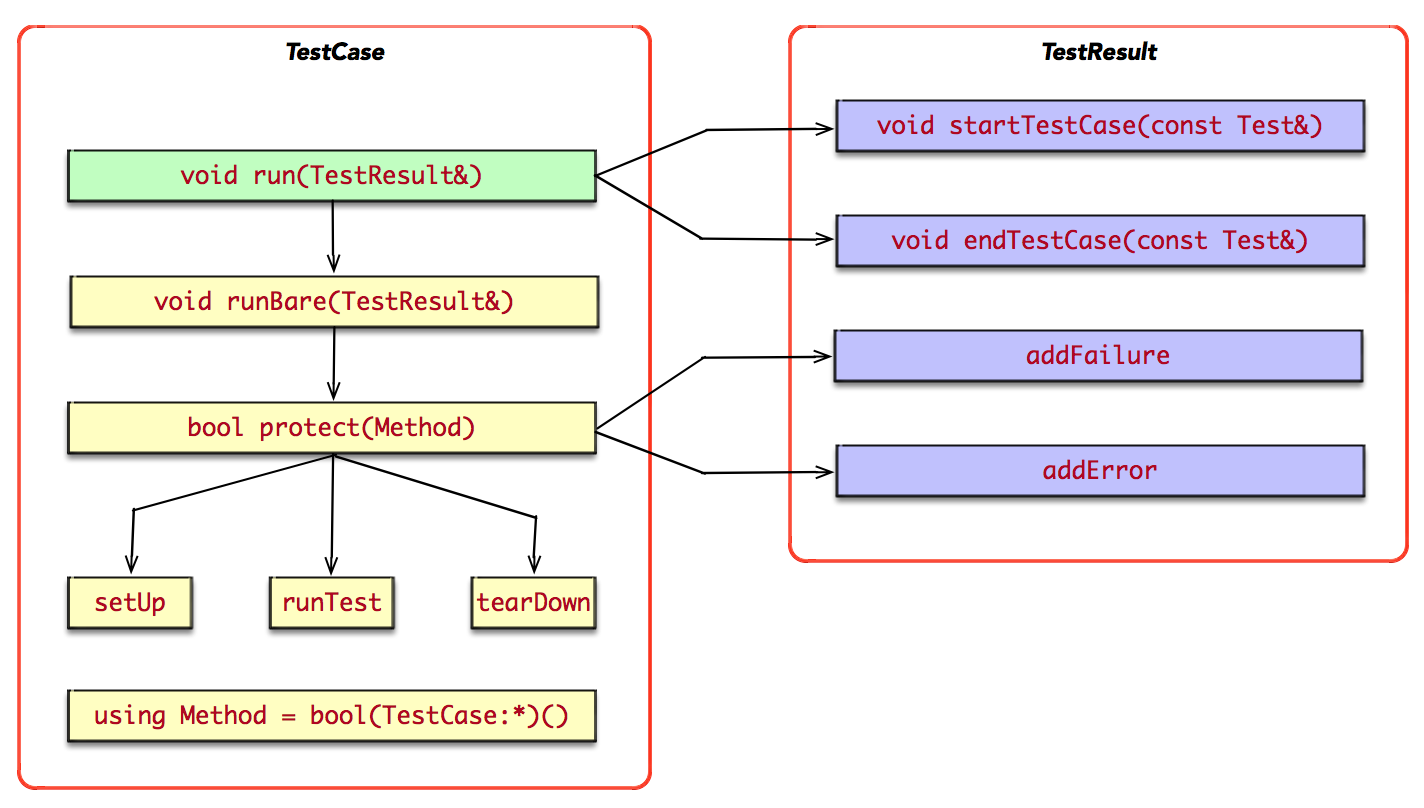
\includegraphics[width=1.0\textwidth]{figures/xunit/coupling-1.png}
\caption{重构之前}
 \label{fig:coupling-1}
\end{figure}

根据迪米特法则,将\ascii{TestCase::protect}搬迁至\ascii{TestResult::protect}。一方面,\ascii{TestResult}暴露给\ascii{TestCase}接口由\ascii{2}减少至\ascii{1},缓解了\ascii{TestCase}对\ascii{TestResult}的耦合关系。另一方面,实现\ascii{TestResult::addFailure, TestResult::addError}的私有化,使得\ascii{TestResult}取得更好的封装特性。

\begin{figure}[H]
\centering
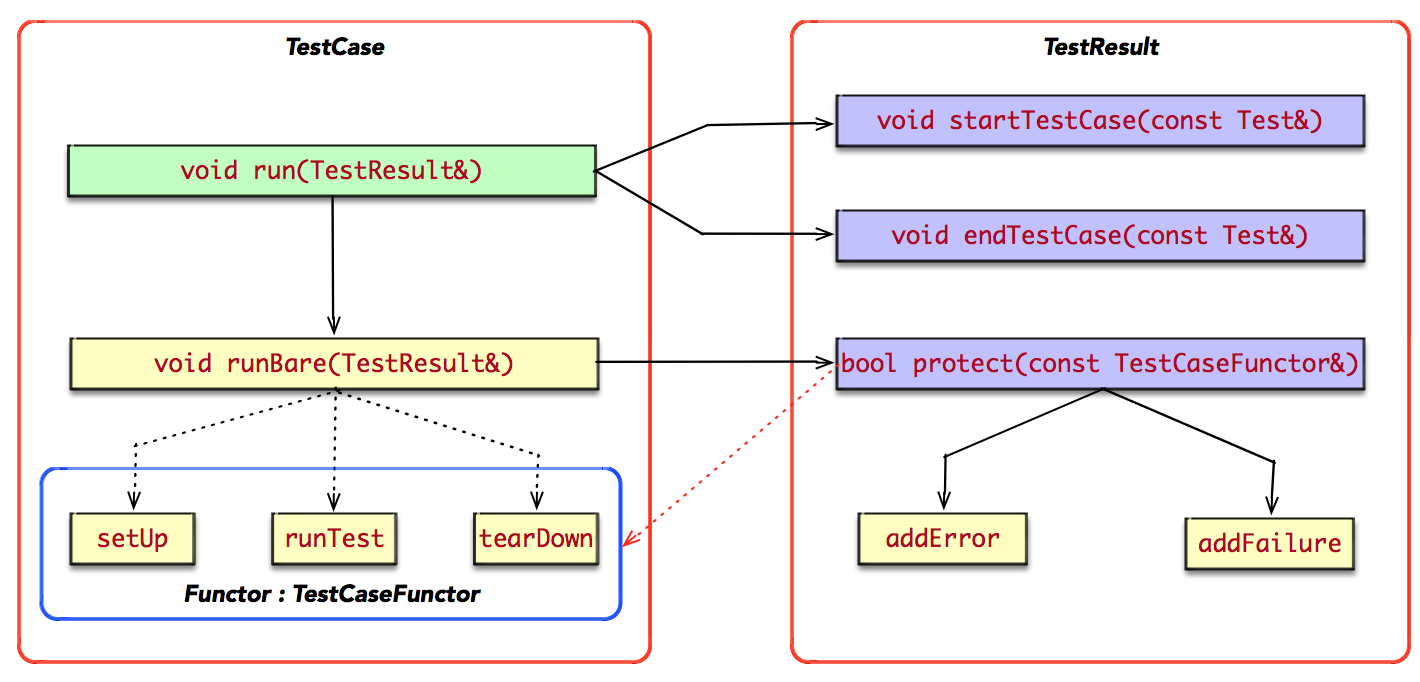
\includegraphics[width=1.0\textwidth]{figures/xunit/decoupling-1-1.png}
\caption{重构之后}
 \label{fig:decoupling-1-1}
\end{figure}

解耦的关键在于抽象接口\ascii{TestCaseFunctor}。在没有破坏\ascii{TestCase}既有封装特性的前提下,使得\ascii{TestResult::protect}不再依赖于具体的\ascii{TestCase::setup, TestCase::runTest, TestCase::tearDown}。

\begin{figure}[H]
\centering
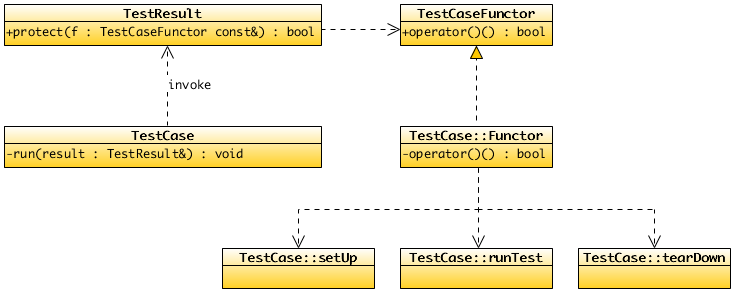
\includegraphics[width=1.0\textwidth]{figures/xunit/test-case-functor-1.png}
\caption{关键抽象: TestCaseFunctor}
 \label{fig:test-case-functor-1}
\end{figure}

\end{content}

% \section{彻底解耦}

% \begin{content}

% 宏函数\ascii{PROTECT}提高了\ascii{TestCase::run}主干逻辑的表达力,但是没有掩盖\ascii{TestCase::run}的主干逻辑与\ascii{TestResult}更亲密的基本事实真相。按照迪米特法则,\ascii{TestCase::run}的主干逻辑应该搬迁至\ascii{TestResult},使得\ascii{TestCase::protect}私有化。

% \subsection{关键抽象}

% \subsubsection{抽象接口:TestCaseProtector}

% \begin{nodiff}
%  \begin{c++}
% struct TestCaseFunctor;

% struct TestCaseProtector {
%   virtual bool protect(const TestCaseFunctor&) = 0;
%   virtual ~TestCaseProtector() {}
% }; 
%  \end{c++}
% \end{nodiff}

% \subsubsection{抽象接口:BareTestCase}

% \begin{nodiff}
%  \begin{c++}
% struct TestCaseProtector;

% struct BareTestCase {
%   virtual void runBare(TestCaseProtector&) = 0;
%   virtual ~BareTestCase() {}
% };
%  \end{c++}
% \end{nodiff}

% \end{content}



